\documentclass[12pt]{article}
\usepackage{lingmacros}
\usepackage{tree-dvips}
\usepackage{graphicx}
\usepackage{grffile}
\usepackage{cite}
\usepackage{float}

\begin{document}
\title{Notes for the Collaboration and competition project}
\date{2018\\ November}
\author{Raphael Gross}
\maketitle




\section{Introduction}
This is the third project of the Udacity DRL course. My goal for this project is to get a better understanding of multi-agents environments using deep reinforcement learning. I implemented some variations of the last Deep Deterministic Policy Gradient (DDPG) \cite{LillicrapHPHETS15} in pytorch. In order to achieve my goal, I explain briefly the main features of the DDPG methods. Then, I describe the Tennis environment used for testing the algorithm. Finally, I show the results I obtained.

I coded the next methods:
\begin{itemize}
\item DDPG: one agent, playing for both side.
\item MA-DDPG: two agents with no shared memory with independant actor-critic.
\item MA-DDPG: two agents with shared memory  with independant actor-critic.
\end{itemize}

\section{State of the Art for DDPG}

I used the DDPG algorithm to solve the Tennis environment. DDPG is a model-free, off-policy actor-critic algorithm that enables solving continuous action environment. 
DDPG is based on the deterministic policy gradient or DPG \cite{LHDWR14}.
DDPG has a parametrized actor function $\mu(s|{\theta}^{\mu})$ which specifies the current policy by deterministically mapping states to a specific action while the critic $Q(s,a)$ is learned using the Bellman equation.

DDPG uses some of the advantages of DQN \cite{mnih2015humanlevel} such as sample replay and the target network.
Sample replay reduces correlations between sample. The replay buffer is constitued of tuples $(s,a,r,s')$  with $s$ the observations, $a$ actions, $r$ rewards and $s'$ the new states.
I stock the interaction between agents and the environment in the same replay buffer without distinction.

The DDPG model like DQN\cite{mnih2015humanlevel} uses a target network adapted to actor-critic and soft target updates for the network weights. We have an actor target $mu'$ and a critic target $Q'$. These two points increase the stability of the network and let it learn the action-value function. 

The principal issue in continuous action space is exploration. I define the exploration policy as the sum of the policy $\mu$ and some noise function $\mathcal{N}$ obtained using the Ornstein-Uhlenbeck process.


\section{Testing environment}
The environment I used to train and test my agent is called Tennis. In this environment, two agents play tennis while controlling rackets. The objective is to make as many passes as possible. To achieve this objective, they need to pass the ball over a net without letting the ball touch the ground or shooting the ball out of the boundaries. It is, therefore, a collaborative environment. For each successful pass, the agent gets a reward of +0.1. If the agent fault the ball, a reward of -0.01 is attributed.

The observation space is composed of 24 variables and each action is determined by a vector of dimension 2 corresponding to going forward or backward and jump. The action vector values are between -1.0 and 1.0.

For this project, I will use the multi-agent Unity environment. This environment is composed of 2 identical agents. Each of them is on one side of the tennis field. The task is episodic. After each episode, each agent gets a reward without discounting.  In order to solve the environment, the average maximum score needs to be greater than 0.5 over 100 consecutive episodes.

\begin{center}
\begin{figure}[H]
  \center
  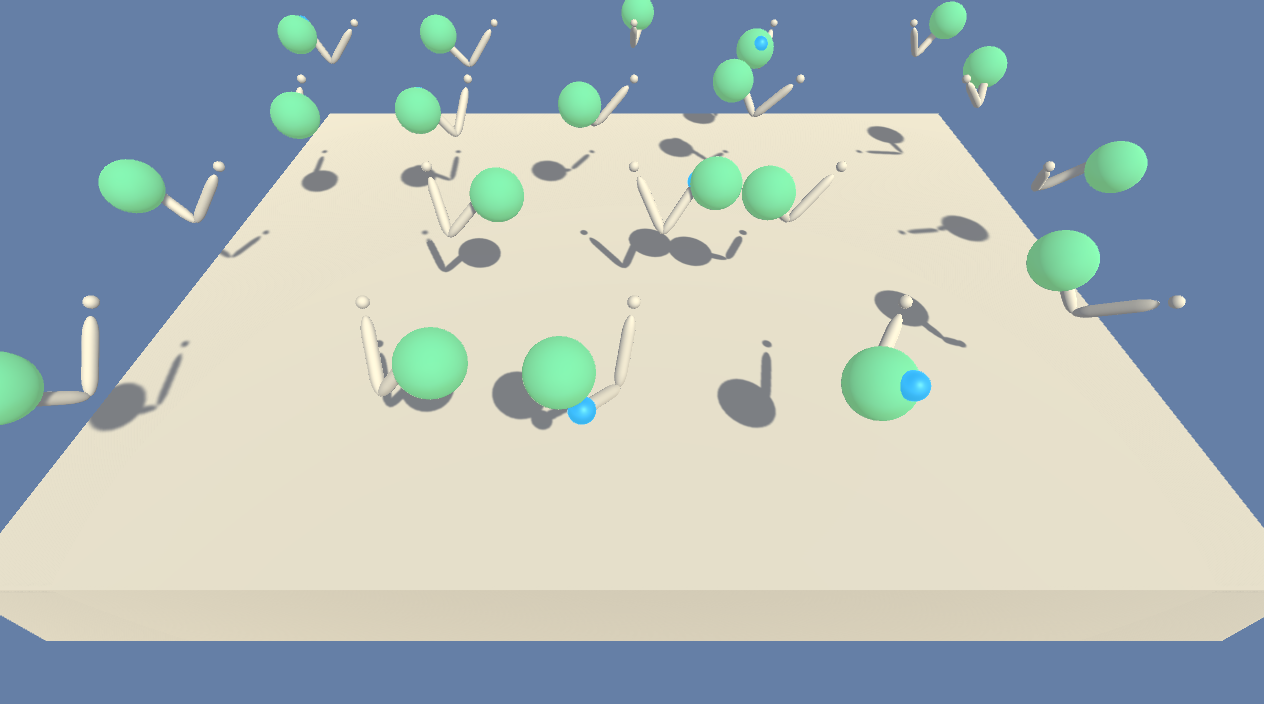
\includegraphics[width=0.7\textwidth]{../PNG/env.png}
  \caption{Tennis environment}
  \label{fig:reacher_environment}
\end{figure}
\end{center}


\section{Results}
\subsection{DDPG model: naive approach} 
The DDPG method is composed of two networks one for the actor and one for the critic. I call this version the naive approach as one agent is playing with himself.

\subsubsection{Actor}
The actor network is composed of linear layers:
\begin{itemize}
\item fc1 : $nn.Linear(state\_size, fc1\_units)$
\item fc2 : $nn.Linear(fc1\_units, fc2\_units)$
\item fc3 : $nn.Linear(fc2\_units, action\_size)$
\end{itemize}

The weight for the first two hidden layers is initialized using a Xavier initialization.
The number of input and output nodes for the hidden layers is defined by the next parameters:

\begin{itemize}
\item $state\_size=24$
\item $fc1\_units=256$
\item $fc2\_units=128$
\item $action\_size=2$
\end{itemize}

In the forward pass, $fc1$ and $fc2$ are combined with a $ReLU$ rectifier. Finally, the policy is given after injecting $fc3$ into a tanh logistic sigmoid function.

\subsubsection{Critic}
The critic-network is composed of linear layers:

\begin{itemize}
\item $fc1 = nn.Linear(state\_size, fc1\_units)$
\item $fc2 = nn.Linear(fc1\_units+action\_size, fc2\_units)$
\item $fc3 = nn.Linear(fc2\_units, 1)$
\end{itemize}
The number of input and output nodes for the hidden layers is defined by the next parameters:

\begin{itemize}
\item $state\_size=24$
\item $fc1\_units=256$
\item $fc2\_units=128$
\item $action\_size=2$
\end{itemize}

The weights for the first two hidden layers are initialized using a Xavier initialization.
The architecture of the critic is a bit unusual. The critic is used to estimate $Q(s, a(\mu))$. But, the action contribution is added to the network only after the first hidden layer.

The authors of the DDPG method\cite{LHDWR14} decided to concatenate the output of the first layer with the action just before the second hidden layer. One possible reason for this choice is to reduce the impact of the critic gradient on the actor computation during the backpropagation.


\begin{itemize}
\item $x\_s   = F.relu(self.fc1(state))$
\item $x\_s\_a = torch.cat((x\_s, action), dim=1)$
\item $x\_s\_a = F.relu(self.fc2(x\_s\_a))$
\item $Q\_s\_a  = self.fc3(x\_s\_a)$
\end{itemize}

\subsection{Parameters}
The best result I obtained for the DDPG method was with the next parameters values:

\begin{itemize}
\item MEMORY SIZE = int(1e5) (replay buffer size)
\item BATCH SIZE = 128  (minibatch size)
\item GAMMA = 0.99  (discount factor)
\item TAU = 1e-3  (parameter value used for the soft update of the target weights)
\item LR\_ACTOR = 8e-5  (learning rate for actor)
\item LR\_CRITIC = 8e-5  (learning rate for critic)
\item UPDATE EVERY = 1  (how often the target network is updated)
\end{itemize}


\subsection{Score}
The maximum score is defined as the highest score between agents. The score is the sum of all the rewards an agent obtained during an episode. For the naive approach, we have one agent playing with himself. So we still have two scores: one for "left side" and one for the "right side" of the net.

In Figure ~\ref{fig:ddpg}, I plotted the maximum score obtained by the agents at each episode. 
To solve the environment, the agent needs to have an average score of 0.5 or above over 100 episodes. The algorithm took 1486 episodes to solve the environment with an average score for the last 100 episodes of 0.516. The score for the last episode is 1.9 which corresponds to 19 successful passes. Also, the agent manages to reach at multiple times a score of 2.5 during the last 100 episodes.

\begin{center}
\begin{figure}[H]
  \center
  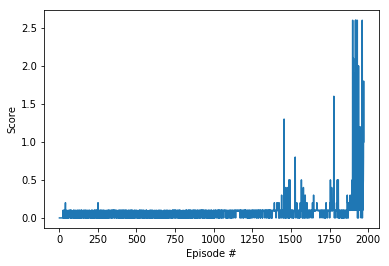
\includegraphics[width=0.7\textwidth]{../PNG/ddpg.png}
  \caption{Maximum score par episode}
  \label{fig:ddpg}
\end{figure}
\end{center}


\subsection{MA-DDPG model: no shared memory} 
In this section, I use two independent agents. They do not share memory such as state, action or observation and both of them use the baseline DDPG algorithm.

In Figure ~\ref{fig:ma_ddpg_1}, I plotted the maximum score obtained by the agents at each episode. 
The algorithm took 3864 episodes to solve the environment with an average score for the last 100 episodes of 0.523. The score for the last episode is 2.60 which corresponds to 26 successful exchanges. Also, the agents manage to reach at multiple times a score of 2.6 during the last few episodes.

\begin{center}
\begin{figure}[H]
  \center
  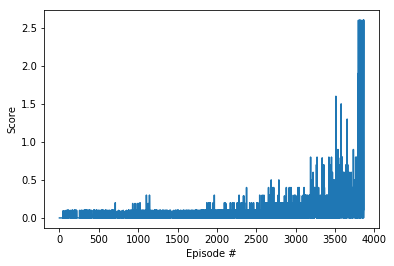
\includegraphics[width=0.7\textwidth]{../PNG/ma_ddpg_1.png}
  \caption{Maximum score par episode}
  \label{fig:ma_ddpg_1}
\end{figure}
\end{center}

\subsection{MA-DDPG model: with shared memory} 
In this section, I use two independent agents. They share memory such as state, action or observation and both of them use the baseline DDPG algorithm. However, the actor-critic only take the input of its associated agent.

In Figure ~\ref{fig:ma_ddpg_2}, I plotted the maximum score obtained by the agents at each episode. 
The algorithm took 2504 episodes to solve the environment with an average score for the last 100 episodes of 0.503. The score for the last episode is 2.60 which corresponds to 26 successful exchanges. Also, the agents manage to reach at multiple times a score of 2.6 during the last few episodes.

\begin{center}
\begin{figure}[H]
  \center
  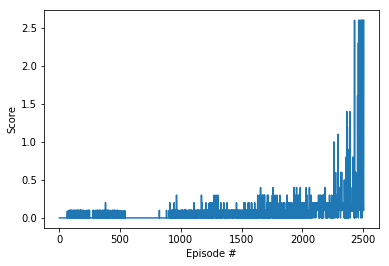
\includegraphics[width=0.7\textwidth]{../PNG/ma_ddpg_2.png}
  \caption{Maximum score par episode}
  \label{fig:ma_ddpg_2}
\end{figure}
\end{center}

\subsection{Future improvement}
For now, I only covered the DDPG\cite{LillicrapHPHETS15} algorithm and some basic variations. But, my ambition is to finish the MADDPG method\cite{NIPS20177217} I started to implement. I also want to try the MADDPG on a more richer project such as the football project where the environment is not only collaborative between players of the same team but also competitive between teams.

\bibliography{report}
\bibliographystyle{plain}

\end{document}


